\documentclass[border=2pt]{standalone}
\usepackage[T1]{fontenc}
\usepackage{helvet}
\renewcommand{\familydefault}{\sfdefault}
\usepackage{tikz}
\usetikzlibrary{arrows.meta,calc}

\definecolor{ink}{HTML}{0F172A}
\definecolor{muted}{HTML}{64748B}
\definecolor{line}{HTML}{CBD5E1}
\definecolor{panel}{HTML}{FBFDFF}
\definecolor{gm}{HTML}{334155}
\definecolor{bold}{HTML}{B91C1C}
\definecolor{boldbg}{HTML}{FEF2F2}
\definecolor{caut}{HTML}{1D4ED8}
\definecolor{cautbg}{HTML}{EFF6FF}
\definecolor{cas}{HTML}{15803D}
\definecolor{casbg}{HTML}{F0FDF4}
\definecolor{grey}{HTML}{94A3B8}
\definecolor{tgreen}{HTML}{5A9E56}
\definecolor{tyellow}{HTML}{C2A83E}
\definecolor{tgray}{HTML}{D7DBE0}

\newcommand{\nametext}[1]{{\fontsize{7.8}{9.2}\selectfont\bfseries\color{ink}#1}}
\newcommand{\roletext}[1]{{\fontsize{6.2}{7.4}\selectfont\color{muted}#1}}
\newcommand{\cardtitle}[1]{{\fontsize{7.2}{8.6}\selectfont\bfseries\color{ink}#1}}
\newcommand{\cardsub}[1]{{\fontsize{6}{7.2}\selectfont\color{muted}#1}}
\newcommand{\panellabel}[1]{{\fontsize{5.9}{6.9}\selectfont\bfseries\color{grey}#1}}
\newcommand{\plabel}[1]{{\fontsize{5.7}{6.7}\selectfont\color{muted}#1}}
\newcommand{\tileletter}[1]{{\fontsize{8}{9}\selectfont\bfseries#1}}
\newcommand{\flowlabel}[1]{{\fontsize{5.2}{6.1}\selectfont\color{muted}#1}}

\begin{document}
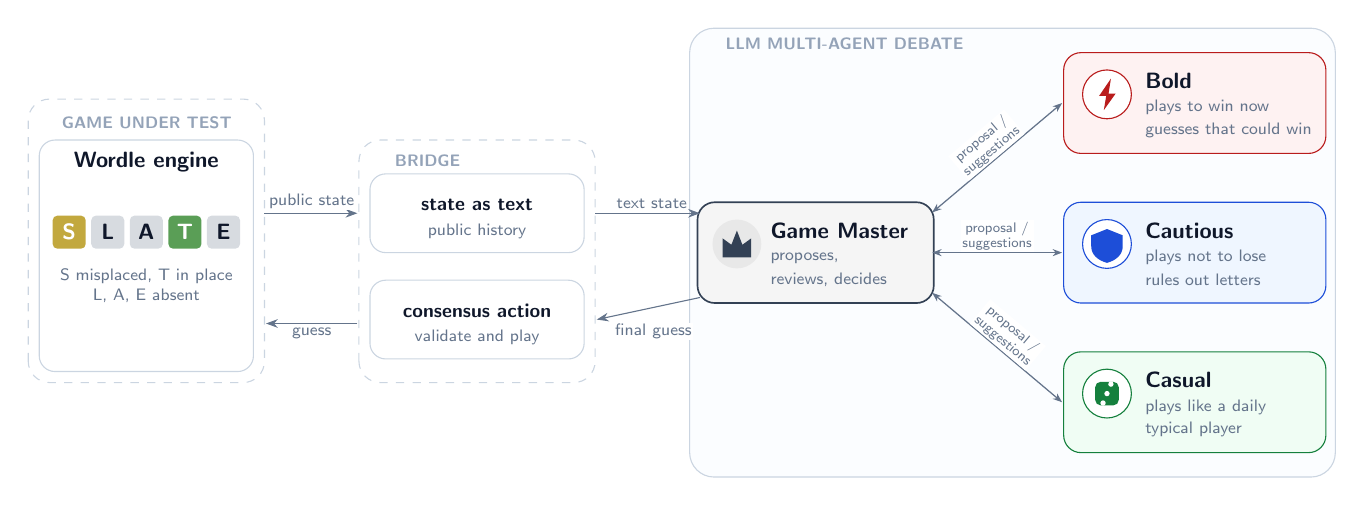
\begin{tikzpicture}[x=1cm,y=1cm,line width=0.4pt]

% ---------- containers ----------
\draw[rounded corners=2.7mm, dashed, line] (0.20,2.20) rectangle (3.20,5.80);
\draw[rounded corners=2.7mm, dashed, line] (4.40,2.20) rectangle (7.40,5.28);
\draw[rounded corners=3.1mm, line, fill=panel] (8.60,1.00) rectangle (16.80,6.70);
\node[anchor=south west, inner sep=0] at (0.62,5.42) {\panellabel{GAME UNDER TEST}};
\node[anchor=south west, inner sep=0] at (4.85,4.94) {\panellabel{BRIDGE}};
\node[anchor=south west, inner sep=0] at (9.05,6.42) {\panellabel{LLM MULTI-AGENT DEBATE}};

% ---------- game under test: one turn ----------
\draw[rounded corners=2mm, line] (0.34,2.34) rectangle (3.06,5.28);
\node[anchor=center, inner sep=0] at (1.70,5.00) {\nametext{Wordle engine}};
\foreach \l/\c/\t [count=\i] in {S/tyellow/white,L/tgray/ink,A/tgray/ink,T/tgreen/white,E/tgray/ink} {
  \pgfmathsetmacro{\x}{0.51+(\i-1)*0.49}
  \fill[\c, rounded corners=0.6mm] (\x,3.90) rectangle ++(0.42,0.42);
  \node[anchor=center, inner sep=0, text=\t] at (\x+0.21,4.11) {\tileletter{\l}};
}
\node[anchor=center, inner sep=0] at (1.70,3.55) {\plabel{S misplaced, T in place}};
\node[anchor=center, inner sep=0] at (1.70,3.30) {\plabel{L, A, E absent}};

% ---------- bridge ----------
\draw[rounded corners=2mm, line] (4.54,3.85) rectangle (7.26,4.85);
\node[anchor=center, inner sep=0] at (5.90,4.46) {\cardtitle{state as text}};
\node[anchor=center, inner sep=0] at (5.90,4.12) {\cardsub{public history}};
\draw[rounded corners=2mm, line] (4.54,2.50) rectangle (7.26,3.50);
\node[anchor=center, inner sep=0] at (5.90,3.11) {\cardtitle{consensus action}};
\node[anchor=center, inner sep=0] at (5.90,2.77) {\cardsub{validate and play}};

% ---------- game master ----------
\draw[rounded corners=2.2mm, draw=gm, line width=0.6pt, fill=gray!8] (8.70,3.21) rectangle (11.70,4.49);
\draw[fill=gray!18, draw=none] (9.20,3.96) circle (0.31);
\fill[gm] (9.02,3.79) -- (9.02,4.03) -- (9.13,3.95) -- (9.20,4.13) -- (9.27,3.95) -- (9.38,4.03) -- (9.38,3.79) -- cycle;
\node[anchor=west, inner sep=0] at (9.62,4.13) {\nametext{Game Master}};
\node[anchor=west, inner sep=0] at (9.62,3.78) {\roletext{proposes,}};
\node[anchor=west, inner sep=0] at (9.62,3.50) {\roletext{reviews, decides}};

% ---------- advisors ----------
% Bold
\draw[rounded corners=2.2mm, draw=bold, fill=boldbg] (13.35,5.11) rectangle (16.68,6.39);
\draw[fill=white, draw=bold] (13.90,5.86) circle (0.31);
\fill[bold] (13.95,6.06) -- (13.80,5.84) -- (13.89,5.84) -- (13.86,5.66) -- (14.01,5.87) -- (13.92,5.87) -- cycle;
\node[anchor=west, inner sep=0] at (14.38,6.03) {\nametext{Bold}};
\node[anchor=west, inner sep=0] at (14.38,5.69) {\roletext{plays to win now}};
\node[anchor=west, inner sep=0] at (14.38,5.40) {\roletext{guesses that could win}};
% Cautious
\draw[rounded corners=2.2mm, draw=caut, fill=cautbg] (13.35,3.21) rectangle (16.68,4.49);
\draw[fill=white, draw=caut] (13.90,3.96) circle (0.31);
\fill[caut] (13.90,4.15) -- (14.10,4.07) -- (14.10,3.93) .. controls (14.10,3.82) and (14.01,3.75) .. (13.90,3.72) .. controls (13.79,3.75) and (13.70,3.82) .. (13.70,3.93) -- (13.70,4.07) -- cycle;
\node[anchor=west, inner sep=0] at (14.38,4.13) {\nametext{Cautious}};
\node[anchor=west, inner sep=0] at (14.38,3.79) {\roletext{plays not to lose}};
\node[anchor=west, inner sep=0] at (14.38,3.50) {\roletext{rules out letters}};
% Casual
\draw[rounded corners=2.2mm, draw=cas, fill=casbg] (13.35,1.31) rectangle (16.68,2.59);
\draw[fill=white, draw=cas] (13.90,2.06) circle (0.31);
\draw[rounded corners=0.7mm, fill=cas, draw=none] (13.75,1.91) rectangle (14.05,2.21);
\fill[white] (13.85,1.94) circle (0.34mm);
\fill[white] (13.95,2.18) circle (0.34mm);
\fill[white] (13.90,2.06) circle (0.34mm);
\node[anchor=west, inner sep=0] at (14.38,2.23) {\nametext{Casual}};
\node[anchor=west, inner sep=0] at (14.38,1.89) {\roletext{plays like a daily}};
\node[anchor=west, inner sep=0] at (14.38,1.60) {\roletext{typical player}};

% ---------- arrows ----------
\draw[-{Stealth[length=1.5mm,width=1.1mm]}, draw=muted] (3.20,4.35) -- (4.38,4.35);
\node[anchor=south, inner sep=0.4pt, fill=white] at (3.80,4.39) {\plabel{public state}};
\draw[-{Stealth[length=1.5mm,width=1.1mm]}, draw=muted] (4.38,2.95) -- (3.22,2.95);
\node[anchor=north, inner sep=0.4pt, fill=white] at (3.80,2.91) {\plabel{guess}};

\draw[-{Stealth[length=1.5mm,width=1.1mm]}, draw=muted] (7.40,4.35) -- (8.73,4.35);
\node[anchor=south, inner sep=0.4pt, fill=white] at (8.12,4.39) {\plabel{text state}};
\draw[-{Stealth[length=1.5mm,width=1.1mm]}, draw=muted] (8.73,3.28) -- (7.42,3.00);
\node[anchor=north, inner sep=0.4pt, fill=white] at (8.14,2.96) {\plabel{final guess}};

\draw[{Stealth[length=1.2mm]}-{Stealth[length=1.2mm]}, draw=muted, line width=0.45pt]
  (11.68,4.36) -- (13.33,5.75) node[midway, sloped, above, align=center, inner sep=0.6pt, fill=white,
  font=\fontsize{4.8}{5.6}\selectfont\color{muted}] {proposal /\\suggestions};
\draw[{Stealth[length=1.2mm]}-{Stealth[length=1.2mm]}, draw=muted, line width=0.45pt]
  (11.68,3.85) -- (13.33,3.85) node[midway, sloped, above, align=center, inner sep=0.6pt, fill=white,
  font=\fontsize{4.8}{5.6}\selectfont\color{muted}] {proposal /\\suggestions};
\draw[{Stealth[length=1.2mm]}-{Stealth[length=1.2mm]}, draw=muted, line width=0.45pt]
  (11.68,3.34) -- (13.33,1.95) node[midway, sloped, above, align=center, inner sep=0.6pt, fill=white,
  font=\fontsize{4.8}{5.6}\selectfont\color{muted}] {proposal /\\suggestions};

\end{tikzpicture}
\end{document}
